\section{Derivation}
This section is organized as follows, we will first derive a very basic sensing matrix\footnote{Here, we define the sensing matrix to be a matrix that maps sensor readouts to the displacements that we want to measure.}, assuming there's no misalignment in the optical system.
And then, we will derive the general sensing matrix that includes all sorts of misalignment.
Lastly, we will modify the matrix for a folded optical lever configuration.
\subsection{Very basic derivation \label{sec:very_basic_derivation}}
In the simplest case, the beam position $x_1$ (along the incidence plane) is related to the angular displacement $\theta$ by
\begin{equation}
	x_1=\left(2r\right)\theta,
\end{equation}
where $r$ is the lever arm defined by the distance between the reflective surface and the sensing device.
The same beam can be used to measure the longitudinal displacement of the reflective surface, if the light beam has an angle of incidence $\alpha$.
In this case, the beam displacement reads
\begin{equation}
	x_1=\left(2r\right)\theta + \left(2\sin{\alpha}\right)x_L,
	\label{eqn:beam_displacement_l}
\end{equation}
where $x_L$ is the longitudinal displacement of the reflective surface.
As can be seen, equation.~\eqref{eqn:beam_displacement_l} shows a coupled sensor where it reads both the angular displacement and the longitudinal shift.
In KAGRA, some optical levers have a second sensor measuring the beam displacement $x_2$ some distance $d$ behind a convex lens with focal length $f$.
In this case, we obtain the second beam displacement $x_2$ via ray transfer matrices \cite{enwiki:1018856234}
\begin{equation}
	\begin{pmatrix}
		x_2\\
		\cdot
	\end{pmatrix}
	=
	\begin{bmatrix}
		1 & d\\
		0 & 1
	\end{bmatrix}
	\begin{bmatrix}
		1 & 0\\
		-1/f & 1
	\end{bmatrix}
	\begin{bmatrix}
		1 & r_\mathrm{lens} \\
		0 & 1
	\end{bmatrix}
	\begin{pmatrix}
		\left(2\sin{\alpha} \right)x_L\\
		2\theta
	\end{pmatrix},
\end{equation}
where $r_\mathrm{lens}$ is the distance between the reflective surface and the lens.
This gives
\begin{equation}
	x_2 = \left(2\sin\alpha\right)\left(1-\frac{d}{f}\right)x_L + 2\left[\left(1-\frac{d}{f}\right)r_\mathrm{lens}+d\right]\theta. 
	\label{eqn:beam_displacement_lens_1}
\end{equation}
Furthermore, we can place the second beam displacement sensor distance behind the lens.
So, if we set
\begin{equation}
	d=\frac{r_\mathrm{lens}f}{r_\mathrm{lens}-f},
	\label{eqn:d}
\end{equation}
then the angular coupling, i.e. the second term in Eqn.~\eqref{eqn:beam_displacement_lens_1}, becomes zero, effectively making the second beam displacement sensor a ``length'' (length as in longitudinal displacement) sensing device.
If Eqn.~\eqref{eqn:d} is satisfied, then the beam displacement measured by the second senor reads
\begin{equation}
	x_2 = \left(\frac{-2f\sin\alpha}{r_\mathrm{lens}-f}\right)x_L.
	\label{eqn:x2}
\end{equation}
Now, if we put Eqn.~\eqref{eqn:beam_displacement_l} and Eqn.~\eqref{eqn:x2} in a matrix form, we can obtain the sensing matrix, i.e.
\begin{equation}
	\begin{pmatrix}
		x_L\\
		\theta
	\end{pmatrix}
	=
	\begin{bmatrix}
		2\sin\alpha & 2r\\
		\frac{-2f\sin\alpha}{r_\mathrm{lens}-f} & 0
	\end{bmatrix}^{-1}
	\begin{pmatrix}
		x_1\\
		x_2
	\end{pmatrix}
\end{equation}
Then, from here, we can diagonalize\footnote{
Consider a model $\vec{y}=\mathbf{C}\vec{x}$, where $\vec{y}$ are the measurements, and $\vec{x}$ are the states.
The goal is to define another measurement basis $\vec{y'}$ such that $\vec{y'}=\mathbf{C'}\vec{x}$, where $\mathbf{C'}$ is a diagonal matrix.
It's obvious that If we define $\vec{y'}\equiv\mathbf{C}^{-1}\vec{y}$, then $\mathbf{C'}$ becomes the identity, which is a diagonal matrix.
Therefore, we define $\mathbf{C}^\mathrm{-1}$ to be the sensing matrix, which maps sensor measurements to the displacements of the reflective surface.
}
the sensors.

\subsection{Optical levers in KAGRA}
Before diving into the discussion of misalignment, let's rewrite the matrix so it's closer to what we see in KAGRA.

In KAGRA, we have two beam displacement sensors\footnote{Some only has one, e.g. MCo.}, tilt-sensing QPD and length-sensing QPD. They are analogous to the first and second beam position sensors in Sec.~\ref{sec:very_basic_derivation}, respectively.
Each QPD has two readouts, the horizontal and the vertical displacement of the beam spot, denoted ($x_\mathrm{tilt}$, $y_\mathrm{tilt}$), and ($x_\mathrm{len}$, $y_\mathrm{len}$) for tilt-sensing QPD and length-sensing QPD respectively.
Here, note that the displacements sensed by the QPDs are not, in general, parallel to the global horizontal or vertical plane, as the QPDs are virtually placed orthogonal to the beam.
We are particularly interested in the optics' longitudinal $x_L$, pitch $\theta_P$, and yaw $\theta_Y$ displacements.
Therefore, the goal is to find a matrix that maps $\vec{x}=\left(x_\mathrm{tilt},\, y_\mathrm{tilt},\, x_\mathrm{len},\, y_\mathrm{len}\right)^T$ to longitudinal displacement, pitch angle, and yaw angle $\left(x_L,\, \theta_P,\, \theta_Y\right)^T$.

\begin{figure}[!h]
	\centering
	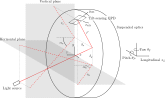
\includegraphics[width=0.7\linewidth]{figures/kagra_optical_lever_3d}
	\caption{Tilt-sensing optical lever setup in KAGRA.}
	\label{fig:kagraopticallever3d}
\end{figure}

A 3D illustration of the a general tilt-sensing optical lever setup is shown in Fig.~\ref{fig:kagraopticallever3d}.
For the current discussion, let's assume that the optical lever is well aligned so the beam spot miscentering at the optics $\delta_x$ and $\delta_y$ are zero.
Now, the lever arm of the optical lever can be an arbitrary vector, i.e. $\vec{r}=r_x\hat{x}+r_y\hat{y}+r_z\hat{z}$.
For the purpose of this discussion, let $\hat{x}$ be a direction aligned to the transverse direction of the main optics, $\hat{y}$ be a direction aligned to the vertical direction of the optics, and $\hat{z}$ be a direction aligned to the longitudinal direction of the optics.
Optical levers in KAGRA are aligned on a horizontal plane (i.e. $r_y=0$), or vertical plane (i.e. $r_x=0$).
But, let's assume that they are not zero.

If we project the beam onto a horizontal plane and a vertical plane (along the normal of the suspended optics), the beams have an incidence angle of $\alpha_h$ and $\alpha_v$ on the horizontal plane and the vertical plane, respectively.
It follows that the lever arm that amplifies the pitch angle is the length of the projection of the lever arm $\vec{r}$ on the vertical plane, $r_v$\footnote{Think of it as a cross-product $\vec{\theta}\times\vec{r}$. For example, for pitch, $-\theta_P\hat{x}\times\left(r_x\hat{x}+r_y\hat{y}+r_z\hat{z}\right) = \theta_P\left(-r_y\hat{z}+r_z\hat{y}\right)$, which is a displacement on the horizontal plane, and $r_v=\sqrt{r_y^2+r_z^2}$ is the corresponding lever arm that amplifies pitch.}.
Similarly, the lever arm amplifying the yaw angle is the length of the projection of the lever arm on the horizontal plane, $r_h$.
Therefore, a rotation in yaw $\theta_Y$ and pitch $\theta_P$ would cause the beam spot at the tip of the lever arm to shift by $\left(2r_h\right)\theta_Y$ and $\left(2r_v\right)\theta_P$, on the horizontal plane and vertical plane respectively.
Meanwhile, a longitudinal shift $x_L$ would cause the beam spot to shift by $\left(2\sin\alpha_h\right)x_L$ and $\left(2\sin\alpha_v\right)x_L$ on the horizontal plane and vertical plane, respectively.
From here, we can write the displacement of the beam spot as measured by the tilt-sensing QPD, placed at some distance $\vec{r}$ from the beam spot at the suspended optics plane.
The beam spot displacement is simply a superposition of that caused by a rotation and a longitudinal shift,
\begin{equation}
	x_\mathrm{tilt} = \left(2r_h\right)\theta_Y + \left(2\sin\alpha_h\right)x_L,
	\label{eqn:x_tilt}
\end{equation}
and
\begin{equation}
	y_\mathrm{tilt} = \left(2r_v\right)\theta_P + \left(2\sin\alpha_v\right)x_L.
	\label{eqn:y_tilt}
\end{equation}

As for the length-sensing QPD, let's assume that beam travels some displacement $\vec{r}_\mathrm{lens}$ from the suspended optics to a convex lens with focal length $f$. Fig.~\ref{fig:kagralengthopticallever3d} shows the length-sensing optical lever setup.
Here, note that the beam in Fig.~\ref{fig:kagralengthopticallever3d} is common to that in Fig.~\ref{fig:kagraopticallever3d}\footnote{In reality, there's a beamsplitter in front of the tilt-sensing QPD to divide the beam into two.}.
\begin{figure}[!h]
	\centering
	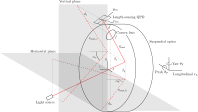
\includegraphics[width=0.7\linewidth]{figures/kagra_length_optical_lever_3d}
	\caption{Length-sensing optical lever setup in KAGRA.}
	\label{fig:kagralengthopticallever3d}
\end{figure}

Let's say the horizontal lever arm from the optics to the convex lens is $r_{\mathrm{lens},h}$.
Again, using ray transfer matrix, we can write down the  beam spot displacement at the length-sensing QPD,
\begin{equation}
	x_\mathrm{len} = \left(2\sin\alpha_h\right)\left(1-\frac{d_h}{f}\right)x_L + 2\left[\left(1-\frac{d_h}{f}\right)r_{\mathrm{lens},h},+d_h\right]\theta_Y,
	\label{eqn:x_len}
\end{equation}
where $d_h$ is the length between the lens and the length-sensing QPD on the horizontal plane, and $f$ is the focal length of the lens.
It follows that when $d_h=\frac{r_{\mathrm{lens},h}f}{r_{\mathrm{lens},h}-f}$, $x_\mathrm{len}$ is decoupled from yaw.
But, $d_h$ is a distance on the horizontal plane.
To get back the length, $d$, we can simply use a similar triangle relationship, as shown in Fig.~\ref{fig:dh},
\begin{equation}
	\begin{split}
	d_\mathrm{yaw} + r_\mathrm{lens} &= \left(d_h+r_{\mathrm{lens} h}\right)\frac{r_\mathrm{lens}}{r_{\mathrm{lens},h}},\\
	d_\mathrm{yaw} &= \left(d_h+r_{\mathrm{lens}, h}\right)\frac{r_\mathrm{lens}}{r_{\mathrm{lens},h}} - r_\mathrm{lens}
	\end{split}
\end{equation}
\begin{figure}[!h]
	\centering
	
\includegraphics[width=0.2\linewidth]{figures/d_h}
	\caption{A similar triangle formed by the beam and it's projection on the horizontal plane (length-sensing QPD path).}
	\label{fig:dh}
\end{figure}
Here, if we set $d=d_\mathrm{yaw}$, then the horizontal readout of the length-sensing QPD $x_\mathrm{len}$ will have no yaw coupling, i.e.
\begin{equation}
	x_\mathrm{len} = \left(\frac{-2f\sin\alpha_h}{r_{\mathrm{lens},h}-f}\right)x_L.
\end{equation}
However, in this case, the vertical readout $y_\mathrm{len}$ is \textbf{not} decoupled from pitch, in general.
Now, if we set $d=d_\mathrm{yaw}$, then, on the vertical plane, $d_v$ reads, again, from similar triangle relation,
\begin{equation}
	\begin{split}
	d_v &= \left(d_\mathrm{yaw}+r_\mathrm{lens}\right)\frac{r_{\mathrm{lens},v}}{r_\mathrm{lens}} - r_{\mathrm{lens},v}\\
	&= \left(d_h+r_{\mathrm{lens},h}\right)\frac{r_{\mathrm{lens},v}}{r_{\mathrm{lens},h}}-r_{\mathrm{lens},v}\\
	&= \left(\frac{r_{\mathrm{lens},h}f}{r_{\mathrm{lens},h}-f}+r_{\mathrm{lens},h}\right)\frac{r_{\mathrm{lens},v}}{r_{\mathrm{lens},h}}-r_{\mathrm{lens},v}\\
	&=\left(\frac{r_{\mathrm{lens},h}}{r_{\mathrm{lens},h}-f}-1\right)r_{\mathrm{lens},v}\\
	&=\frac{r_{\mathrm{lens},v}f}{r_{\mathrm{lens},h}-f}
	\end{split}
\end{equation}
whereas if we want $y_\mathrm{len}$ to be decoupled from pitch, we need to set
\begin{equation}
	d_v = \frac{r_{\mathrm{lens},h}f}{r_{\mathrm{lens},h}-f},
\end{equation}
In general, $r_{\mathrm{lens},h}\neq r_{\mathrm{lens},v}$.
So, we cannot simultaneously decouple pitch and yaw from the length-sensing readout.
And, if we choose to set $d=d_\mathrm{yaw}$, i.e. to minimize yaw coupling, the vertical length-sensing QPD readout reads
\begin{equation}
	\begin{split}
	y_\mathrm{len} &= \left(2\sin\alpha_v\right)\left(1-\frac{d_v}{f}\right)x_L + 2\left[\left(1-\frac{d_v}{f}\right)r_{\mathrm{lens},v}+d_v\right]\theta_P\\
	&= \left(2\sin\alpha_v\right)\left(\frac{r_{\mathrm{lens},h}-r_{\mathrm{lens},v}-f}{r_{\mathrm{lens},h}-f}\right)x_L + 2\left[\left(\frac{r_{\mathrm{lens},h}-r_{\mathrm{lens},v}-f}{r_{\mathrm{lens},h}-f}\right)r_{\mathrm{lens},v} + \frac{r_{\mathrm{lens},v}f}{r_{\mathrm{lens},h}-f}\right] \theta_P\\
	&=\left(2\sin\alpha_v\right)\left(\frac{r_{\mathrm{lens},h}-r_{\mathrm{lens},v}-f}{r_{\mathrm{lens},h}-f}\right)x_L
	+ 2\left[\left(\frac{r_{\mathrm{lens},h}-r_{\mathrm{lens},v}}{r_{\mathrm{lens},h}-f}\right)r_{\mathrm{lens},v}\right] \theta_P.
	\end{split}
	\label{eqn:y_len}
\end{equation}
Here, note that if the length of the projections are equal, i.e. $r_{\mathrm{lens},h}=r_{\mathrm{lens},h}$, then vertical readout of the length-sensing QPD is decoupled from pitch.
This refers to a rather interesting configuration, where the incidence plane of the beam is rotated $45^\circ$ along the $z$-axis with respect to the vertical plane.

Without loss of generality, let's assume arbitrary\footnote{They can't be completely arbitrary. They must be related via the angle between the horizontal plane and the plane of incidence. But, I don't want to introduce that unnecessary parameter.} $d_h$ and $d_v$, and write the sensing matrix.
If we ensemble Eqn.~\eqref{eqn:x_tilt}, \eqref{eqn:y_tilt}, \eqref{eqn:x_len}, and the first line of \eqref{eqn:y_len} into a matrix form, we get
\begin{equation}
	\begin{pmatrix}
		x_L\\
		\theta_P\\
		\theta_Y
	\end{pmatrix}
	=
	\begin{bmatrix}
		2\sin\alpha_h & 0 & 2r_h\\
		2\sin\alpha_v & 2r_v & 0\\
		2\sin\alpha_h\left(1-\frac{d_h}{f}\right) & 0 & 2\left[\left(1-\frac{d_h}{f}\right)r_{\mathrm{lens},h}+d_h\right]\\
		2\sin\alpha_v\left(1-\frac{d_v}{f}\right) &  2\left[\left(1-\frac{d_v}{f}\right)r_{\mathrm{lens},v}+d_v\right] & 0\\
	\end{bmatrix}^{+}
	\begin{pmatrix}
		x_\mathrm{tilt}\\
		y_\mathrm{tilt}\\
		x_\mathrm{len}\\
		y_\mathrm{len}
	\end{pmatrix},
	\label{eqn:sensing_matrix_general}
\end{equation}
where $\begin{bmatrix}\cdot\end{bmatrix}^{+}$ is the pseudoinverse of $\begin{bmatrix}\cdot\end{bmatrix}$, and $\begin{bmatrix}\cdot\end{bmatrix}^{+}\begin{bmatrix}\cdot\end{bmatrix}=\mathbf{I}$.

\subsubsection{Horizontal optical levers \label{sec:horizontal_optical_levers}}
Eqn.~\eqref{eqn:sensing_matrix_general} gives a general relationship between the QPD readouts and the displacements of the optics without misalignments.
It can be drastically simplified if we further assume that the incidence plane is aligned to the horizontal plane (e.g. Type-Bp and Type-A) or the vertical plane (e.g. Type-B). 
For horizontal optical levers, $\alpha_v=0$.
This gives $y_\mathrm{tilt}=\left(2r_v\right)\theta_P$ and $y_\mathrm{len}=2\left[\left(1-\frac{d_v}{f}\right)r_{\mathrm{lens},v}+d_v\right]\theta_P$, which are not independent from each other.
We can choose to omit the readout $y_\mathrm{len}$ and hence the sensing matrix for a horizontal optical lever is
\begin{equation}
	\begin{pmatrix}
		x_L\\
		\theta_P\\
		\theta_Y
	\end{pmatrix}
	=
	\begin{bmatrix}
		2\sin\alpha_h & 0 & 2r_h\\
		0 & 2r_v & 0\\
		\frac{-2f\sin\alpha_h}{r_{\mathrm{lens},h}-f} & 0 & 0
	\end{bmatrix}^{-1}
	\begin{pmatrix}
		x_\mathrm{tilt}\\
		y_\mathrm{tilt}\\
		x_\mathrm{len}
	\end{pmatrix},
	\label{eqn:sensing_matrix_horizontal}
\end{equation}
where we've assumed $d=d_h=\frac{r_{\mathrm{lens},h}f}{r_{\mathrm{lens},h}-f}$.
Note that on a horitonzal setup, the beam is on the horizontal plane so the horizontal lever arm $r_h=r$.
Furthermore, the projection on the vertical plane is simply $r_v=r\cos\alpha_h$.
Similarly, the horizontal arm displacement from the optics to the lens $r_{\mathrm{lens},h}=r_\mathrm{lens}$.

\subsubsection{Vertical optical levers}
Like in Sec.~\ref{sec:horizontal_optical_levers}, we can write the sensing matrix without further derivation
\begin{equation}
	\begin{pmatrix}
		x_L\\
		\theta_P\\
		\theta_Y
	\end{pmatrix}
	=
	\begin{bmatrix}
		0 & 0 & 2r_h\\
		2\sin\alpha_v & 2r_v & 0\\
		\frac{-2f\sin\alpha_v}{r_{\mathrm{lens},v}-f} & 0 & 0
	\end{bmatrix}^{-1}
	\begin{pmatrix}
		x_\mathrm{tilt}\\
		y_\mathrm{tilt}\\
		y_\mathrm{len}
	\end{pmatrix},
	\label{eqn:sensing_matrix_vertical}
\end{equation}
where we've set $d=d_v=\frac{r_{\mathrm{lens},v}f}{r_{\mathrm{lens},v}-f}$.
Again, for a vertical setup, $r_v=r$, $r_h=r\cos\alpha_v$, and $r_{\mathrm{lens},v}=r_\mathrm{lens}$.

\subsubsection{Short summary}
We have derived the sensing matrix, Eqn.~\eqref{eqn:sensing_matrix_general}, assuming no misalignment, for a general optical lever setup with a tilted incidence plane.
From that, we reduced the general matrix to Eqn.~\eqref{eqn:sensing_matrix_horizontal} and \eqref{eqn:sensing_matrix_vertical}, which corresponds to the sensing matrix for a horizontal optical lever setup and vertical optical lever setup, respectively.
In general, the angle of incidence, arm lengths, and focal length are known.
Therefore, Eqn.~\eqref{eqn:sensing_matrix_horizontal} and \eqref{eqn:sensing_matrix_vertical} can be used as initial sensing matrices for the Type-Bp/Type-A and Type-B optical levers, respectively.


\subsection{Misalignment}

